\documentclass[10pt]{article}
\usepackage{amsmath, amssymb, amsfonts, mathtools}
\usepackage{pgfplots}
\pgfplotsset{compat=1.16}

\begin{document}

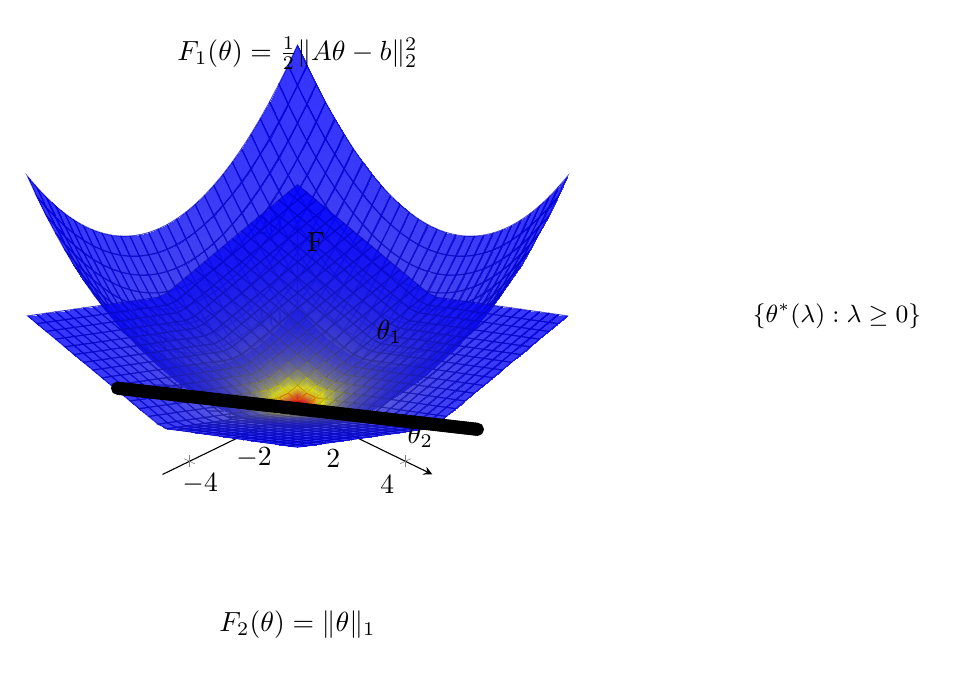
\begin{tikzpicture}
    \begin{axis}[
        axis lines=center,
        xlabel=$\theta_2$,
        ylabel=$\theta_1$,
        zlabel=F,
        xmin=-5,xmax=5,
        ymin=-5,ymax=5,
        zmin=0,zmax=20,
        domain=-5:5,
        y domain=-5:5,
        samples=30,
        grid=major,
        view={45}{45},
        clip=false
    ]
        % Smooth objective function F1
        \addplot3 [
            surf,
            shader=faceted interp,
            z buffer=sort,
            point meta={1/(sqrt(2)*(sqrt(x^2+y^2)+sqrt(x^2/9+y^2/9)))-1},
            color=black,
            opacity=0.7,
            fill opacity=0.8,
        ] {(x^2+y^2)/2};
        
        % Non-smooth objective function F2
        \addplot3 [
            surf,
            shader=faceted interp,
            z buffer=sort,
            point meta={1/(sqrt(2)*(sqrt(x^2+y^2)+sqrt(x^2/9+y^2/9)))-1},
            color=black,
            opacity=0.7,
            fill opacity=0.8,
        ] {abs(x)+abs(y)};
        
        % Regularization path (theta*(lambda))
        \addplot3 [
            mark options={black, thick},
            mark=*,
            domain=-5:5,
            samples=200,
            red,
            thick,
            samples y=0,
            variable=\x,
        ] ({\x},{(1/3)*\x},{\x/2});
        
        % Equations for labels
        \node at (axis cs:-10,10,10) {$F_1(\theta) = \frac{1}{2}\|A\theta - b\|_2^2$};
        \node at (axis cs:10,-10,5) {$F_2(\theta) = \|\theta\|_1$};
        \node at (axis cs:10,10,10) {\small$\{\theta^*(\lambda): \lambda \geq 0\}$};
    \end{axis}
\end{tikzpicture}

\end{document}